\documentclass[]{deedy-resume-openfont}
\usepackage{fancyhdr}
 
\pagestyle{fancy}
\fancyhf{}

\usepackage{graphicx}
\usepackage{tikzpagenodes}
\usepackage[demo]{graphicx}
\usepackage{subfig}
\usepackage{hyperref}
 
\begin{document}

% \lastupdated

\begin{minipage}[t]{0.32\textwidth} 

\namesection{}{Kirill Artemov}{\urlstyle{same}\href{mailto:kaartemov@gmail.com}{kaartemov@gmail.com}}


\begin{tikzpicture}[remember picture,overlay,shift={(current page.north east)}]
    \node[anchor=north east,xshift=-1cm,yshift=-1cm]{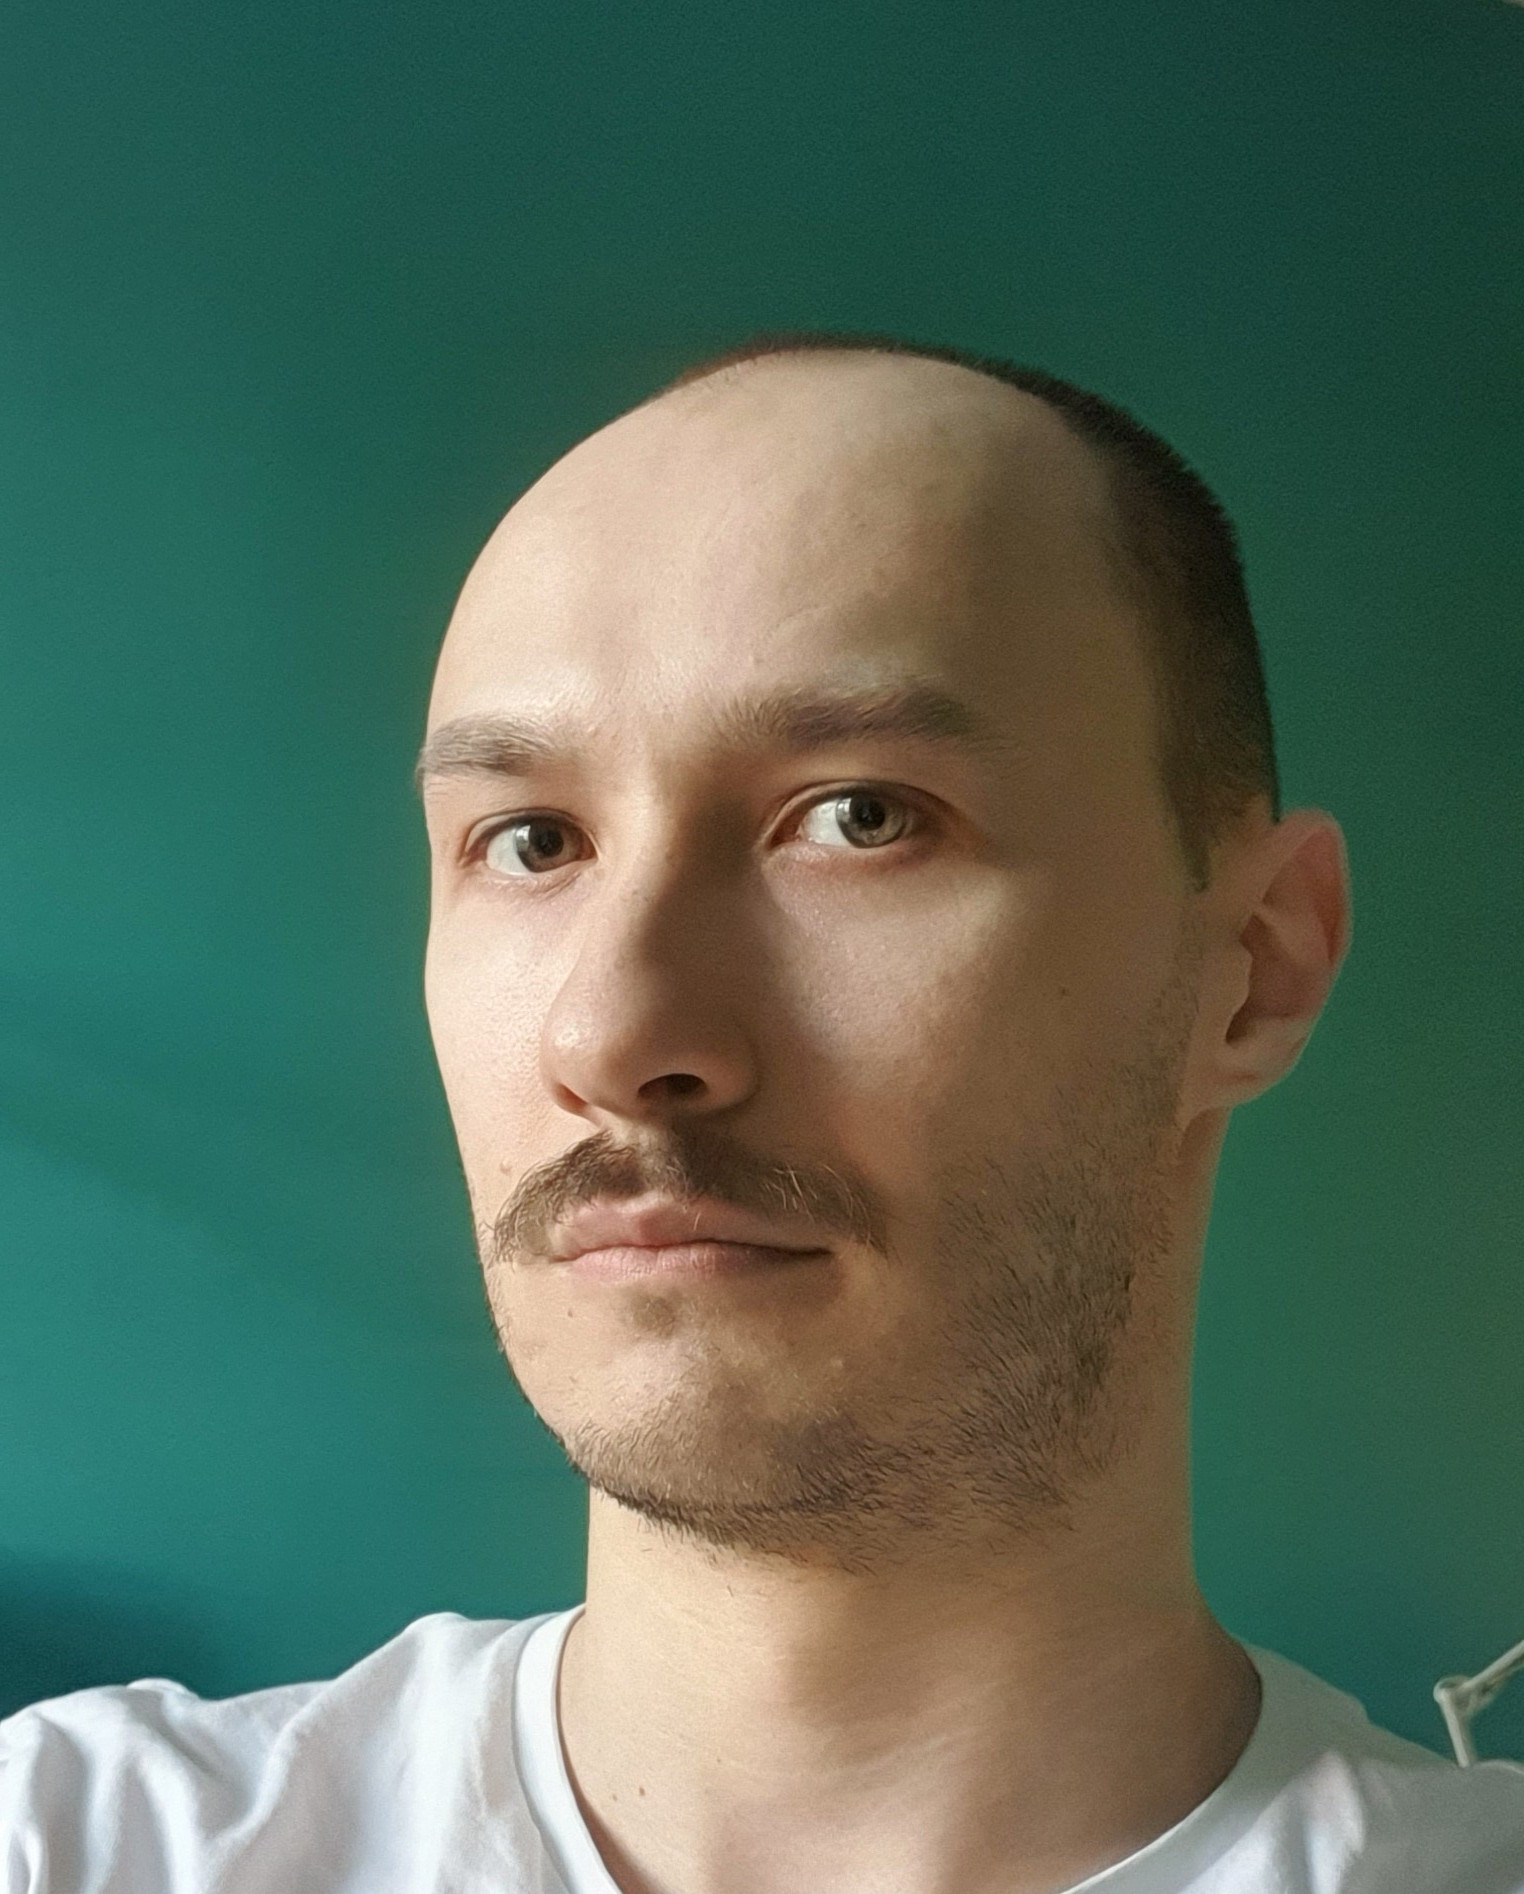
\includegraphics[width=3cm]{me.jpg}};
\end{tikzpicture}


\section{Education} 

\subsection{PhD in Engineering}
\descript{ITMO University}
\location{Thesis: Adaptive reactive and proactive hybrid control of manipulation robots}
\location{2018-2022 | Saint-Petersburg, Russia}
\sectionsep

\subsection{MS in Robotics}
\descript{ITMO University}
\location{Thesis: Robotic system for grasping moving objects}
\location{2016-2018 | Saint-Petersburg, Russia}
\sectionsep

\subsection{BS in Device Engineering}
\descript{KSTU}
\location{Thesis: Development of metrological software for generators of special signals}
\location{2010-2014 | Karaganda, Kazakhstan}
\sectionsep


%%%%%%%%%%%%%%%%%%%%%%%%%%%%%%%%%%%%%%
%     LINKS
%%%%%%%%%%%%%%%%%%%%%%%%%%%%%%%%%%%%%%

\section{Links} 
Github:// \href{https://github.com/kirillin}{\bf kirillin} \\
YouTube://  \href{https://www.youtube.com/@kaartemov}{\bf @kaartemov} \\

%%%%%%%%%%%%%%%%%%%%%%%%%%%%%%%%%%%%%%
%     COURSEWORK
%%%%%%%%%%%%%%%%%%%%%%%%%%%%%%%%%%%%%%

% \section{Coursework}
% \subsection{Graduate}
% Advanced Machine Learning \\
% Open Source Software Engineering \\
% Advanced Interactive Graphics \\
% Compilers + Practicum \\
% Cloud Computing \\
% Evolutionary Computation \\
% Defending Computer Networks \\
% Machine Learning \\
% \sectionsep

% \subsection{Undergraduate}
% Information Retrieval \\
% Operating Systems \\
% Artificial Intelligence + Practicum \\
% Functional Programming \\
% Computer Graphics + Practicum \\
% {\footnotesize \textit{\textbf{(Research Asst. \& Teaching Asst 2x) }}} \\
% Unix Tools and Scripting \\

%%%%%%%%%%%%%%%%%%%%%%%%%%%%%%%%%%%%%%
%     SKILLS
%%%%%%%%%%%%%%%%%%%%%%%%%%%%%%%%%%%%%%

\section{Skills}
% \subsection{Programming}
% \location{Over 5000 lines:}
Python\textbullet{}
C++\textbullet{}
Bash\textbullet{}
Linux\textbullet{}
ROS\textbullet{}
Docker\textbullet{}
Git\textbullet{}
Gazebo/V-rep/pybullet\textbullet{}
Matlab\textbullet{}
KUKA youBot, iiwa\textbullet{}
FESTO Robotino\textbullet{} DJI Tello\textbullet{} INTEL Realsense\textbullet{} Quanser Mechatronics
\sectionsep

\section{Languages}
    English -- fluent\\
    Russian -- mother-tongue
\sectionsep

\section{Hobbies}
    Guitar, Ice-skating, Cars
\sectionsep

\section{Extras}
    Driver license (cat. B),\\
    Citizenship: Kazakhstan
\sectionsep
%%%%%%%%%%%%%%%%%%%%%%%%%%%%%%%%%%%%%%
%
%     COLUMN TWO
%
%%%%%%%%%%%%%%%%%%%%%%%%%%%%%%%%%%%%%%

\end{minipage} 
\hfill
\begin{minipage}[t]{0.66\textwidth} 

\section{Work Experience}
\runsubsection{Research engineer}
\descript{ITMO University}
\location{2017 - Present | Saint-Petersburg, Russia}
\vspace{\topsep} 
\begin{tightemize}
    \item Research in Safety Control of Cobots.
    \item Robots Programming.
    \item Teaching assistant.
\end{tightemize}

\runsubsection{Teacher}
\descript{High School}
\location{2014 - 2016 | Karaganda, Kazakhstan}
\begin{tightemize}
    \item Lego Mindstorms fundamentals.
    \item Robotics Competitions with Lego. 
\end{tightemize}

\runsubsection{Network Engineer}
\descript{High School}
\location{2014 - 2016 | Karaganda, Kazakhstan}
\sectionsep

%%%%%%%%%%%%%%%%%%%%%%%%%%%%%%%%%%%%%%
%     RESEARCH
%%%%%%%%%%%%%%%%%%%%%%%%%%%%%%%%%%%%%%
\vspace{-1.5em}
\section{Selected projects}

\runsubsection{International Laboratory of Biomechatronics and Energy-Efficient Robotics}
\descript{Engigeer}
\location{Saint-Petersburg, Russia}
\vspace{-1em}
\begin{itemize}
    \item 2019-present | \textit{"Ya-Profi" Olympiad in Robotics. Automation testing system developer and head organizer}
    \item 2021-present | \textit{RoboForces platform: automatic testing of simulations in robotics tasks}
    \item 2021-2022 | \textit{Research of AI based methods for robotic perception systems}
    \item 2018-2022 | Design of adaptive methods for sensing, planning and motion control for biomechatronic systems (Russian Science Foundation)
    \item 2019-2020 | Design of algorithms and control systems for service robots using computer vision and human-robot interaction \textit{2019-2020}
    \item 2018-2019 | Development of a quantum platform for secure management of distributed cyber-physical systems 
\end{itemize}
\vspace{-1.5em}
\sectionsep


%%%%%%%%%%%%%%%%%%%%%%%%%%%%%%%%%%%%%%
%     AWARDS
%%%%%%%%%%%%%%%%%%%%%%%%%%%%%%%%%%%%%%

\section{Teaching Experience}

\runsubsection{Course at ITMO University}
\descript{\textit{Foundations of Robotics and Robot programming},}
\descript{Lectures, Seminars, Exercises}
\location{2018-2020, Saint-Petersburg, Russia}
\sectionsep

\runsubsection{Course at ITMO University}
\descript{Dynamics of Robotics Systems}
\descript{Exercises}
\location{2019-2022, Saint-Petersburg, Russia}
\sectionsep

\runsubsection{Workshop}
\descript{WeCORD, Control Systems with ROS}
\descript{\url{https://youtu.be/7V-rgHGb3Tw}}
\location{2019-2022, Saint-Petersburg, Russia}
\sectionsep
\sectionsep

\vspace{-1.5em}
\section{Social work}
\runsubsection{Roboland}
\descript{Judge}
\location{Competition for schoolchildren using Lego}
\location{2014-2018, Kazakhstan}
\vspace{1em}
\runsubsection{I am professional: Robotics league}
\descript{Tasks developer and organizer}
\location{Competition for students using ROS and gazebo}
\location{2019-2022, Russia}

\vspace{1em}
\runsubsection{Robocup@Work, team RED}
\descript{Role: computer vision system developer}
\location{2017-2018, Russia}

\sectionsep

\end{minipage} 

\newpage
%%%%%%%%%%%%%%%%%%%%%%%%%%%%%%%%%%%%%%
%     PUBLICATIONS
%%%%%%%%%%%%%%%%%%%%%%%%%%%%%%%%%%%%%%

\section{Publications} 
\renewcommand\refname{\vskip -1.5em} % Couldn't get this working from the .cls file
\bibliographystyle{abbrv}
\bibliography{publications}
\nocite{*}

\section{Appendix}
\descript{Different videos about my projects}

\begin{figure}[h]
    \centering
    \subfloat[\centering Sorting cell with \textbf{KUKA LWR iiwa (\href{https://youtu.be/F0UuQsvs7Nk}{click})}]{{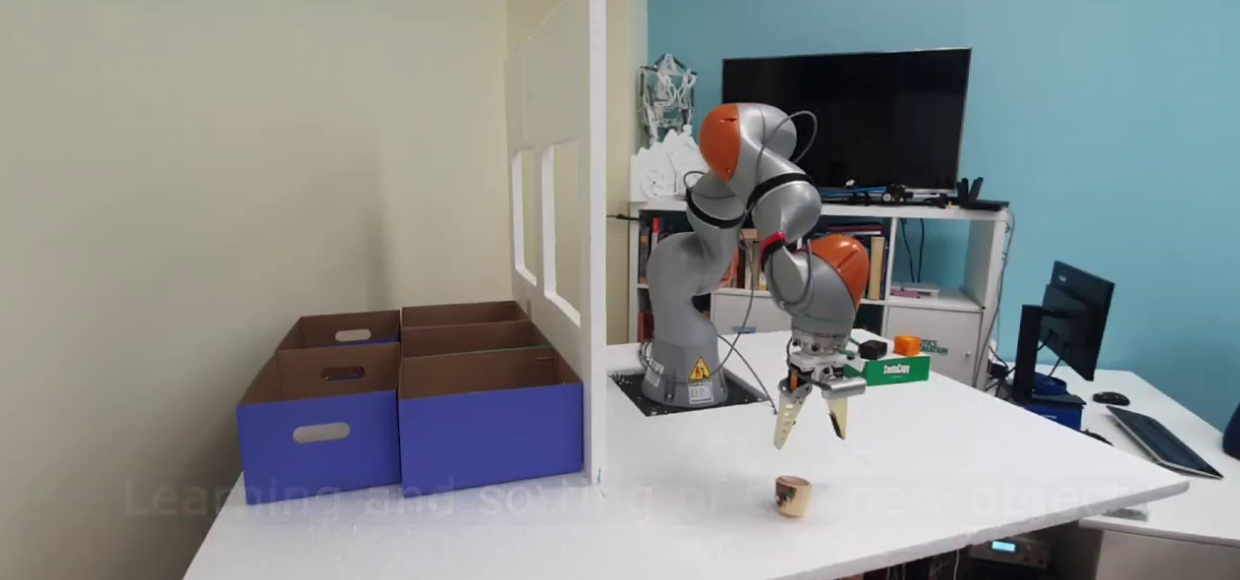
\includegraphics[width=5cm]{figs/grasping.png} }}%
    \quad
    \subfloat[\centering Sorting cell with \textbf{UR5} (\href{https://youtu.be/YyNo43eolho}{click})]{{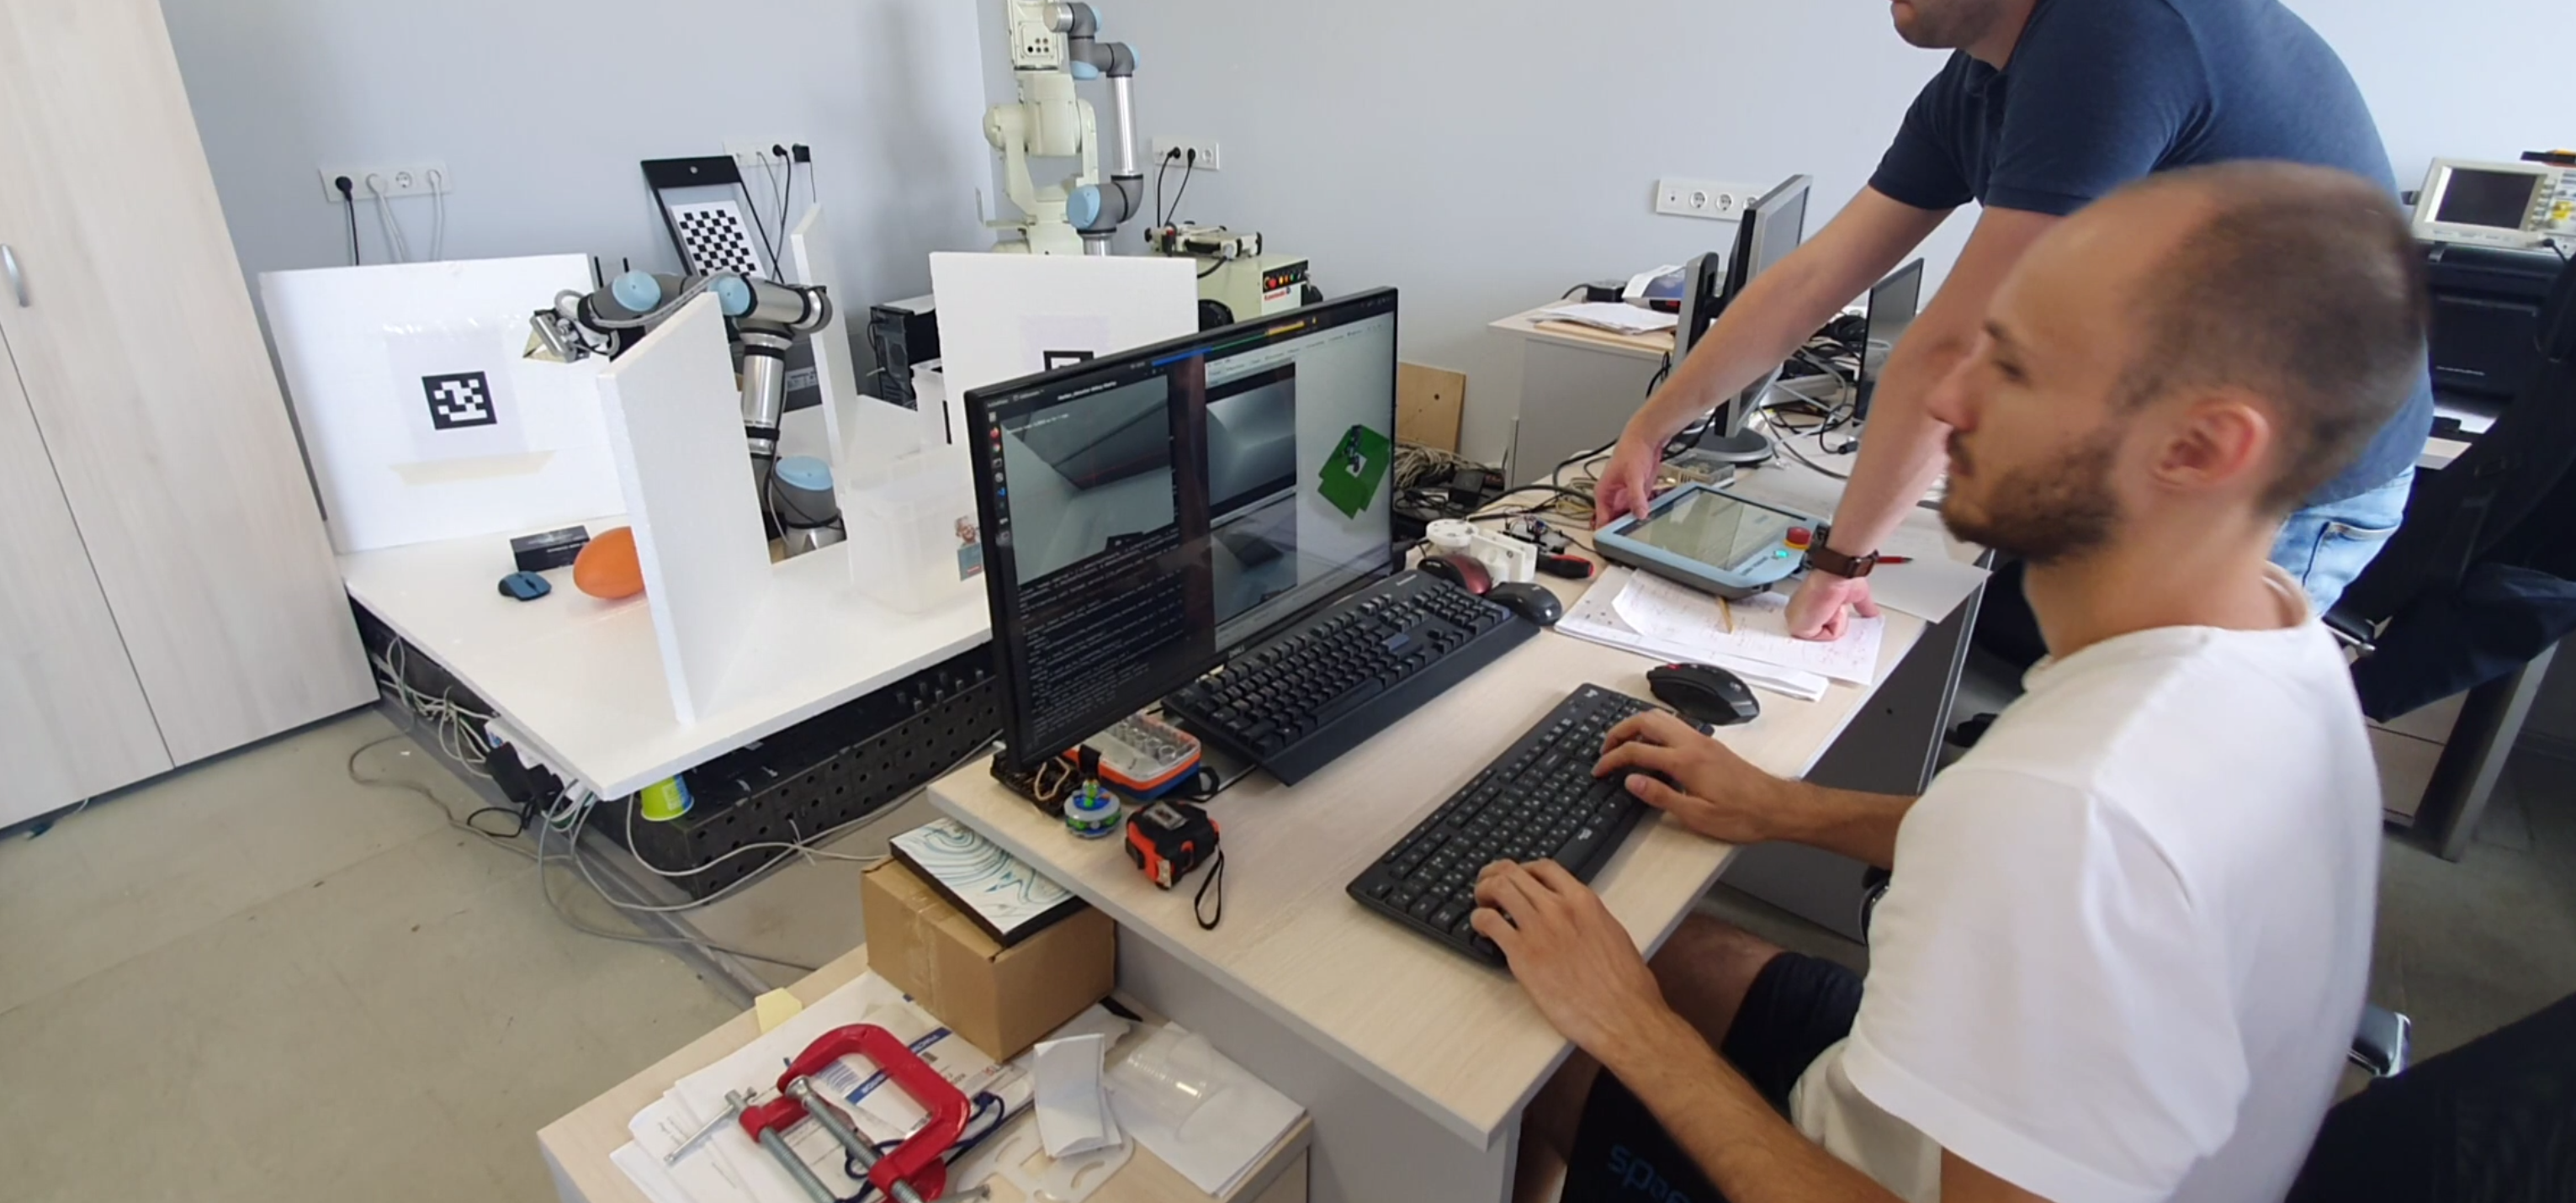
\includegraphics[width=5cm]{figs/grasping_ur.png} }}%
    \quad
    \subfloat[\centering Navigation stack for \textbf{KUKA youBot (\href{https://youtu.be/Ma1Jxzw3y7A}{click})}]{{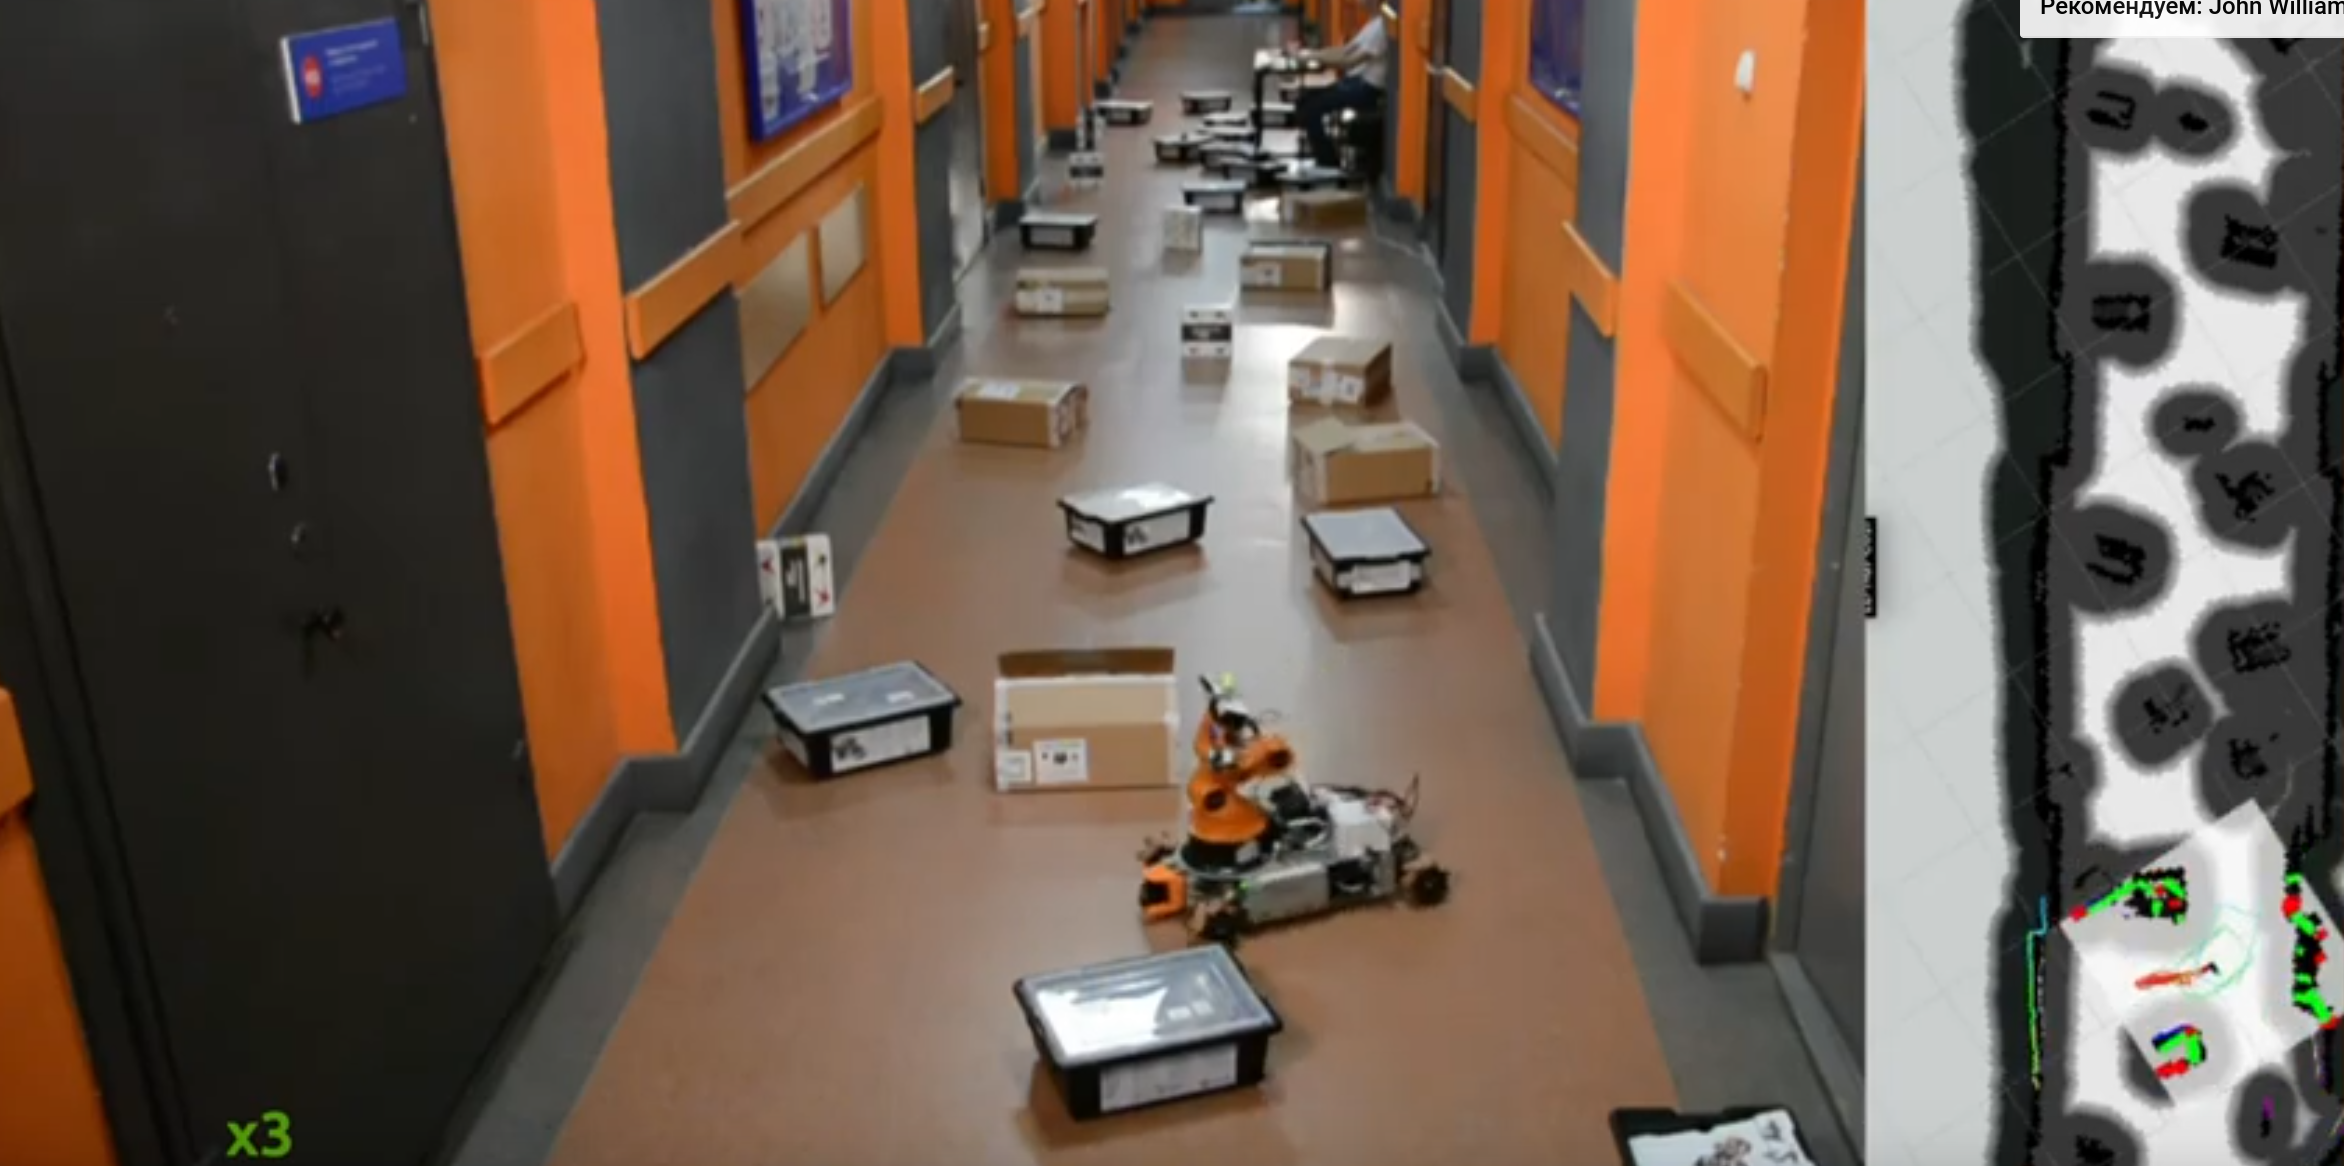
\includegraphics[width=5cm]{figs/gmapping.png} }}%
\end{figure}

\begin{figure}[h]
    \centering
    \subfloat[\centering Visual Servoing for \textbf{KUKA youBot arm (\href{https://youtu.be/UPhpe6U_VrA}{click})}]{{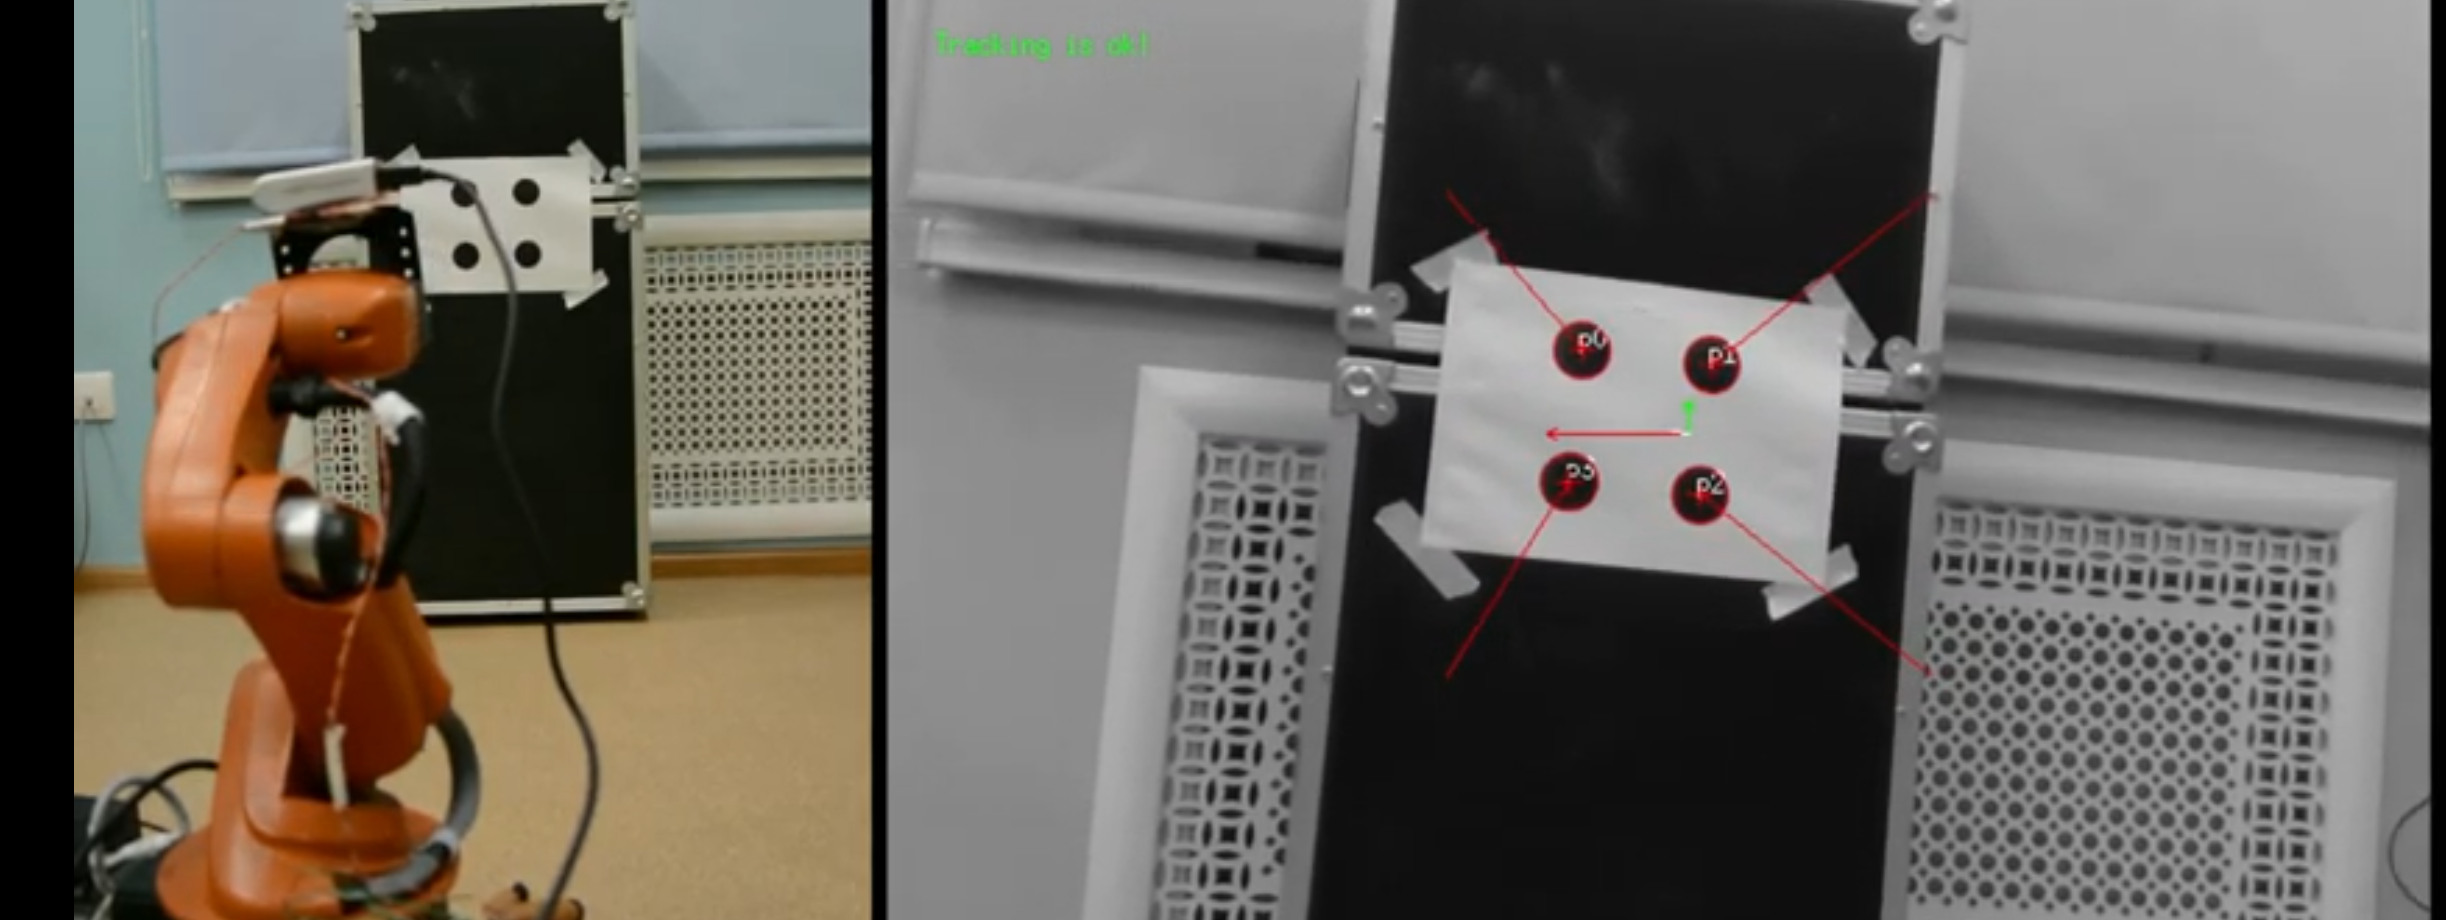
\includegraphics[width=3cm]{figs/visp.png} }}%
    \quad
    \subfloat[\centering Collaborative control of \textbf{KUKA LWR iiwa} and \textbf{Quanser Inverted Pendulum (\href{https://youtu.be/RzPyDXsU6ng}{click})}]{{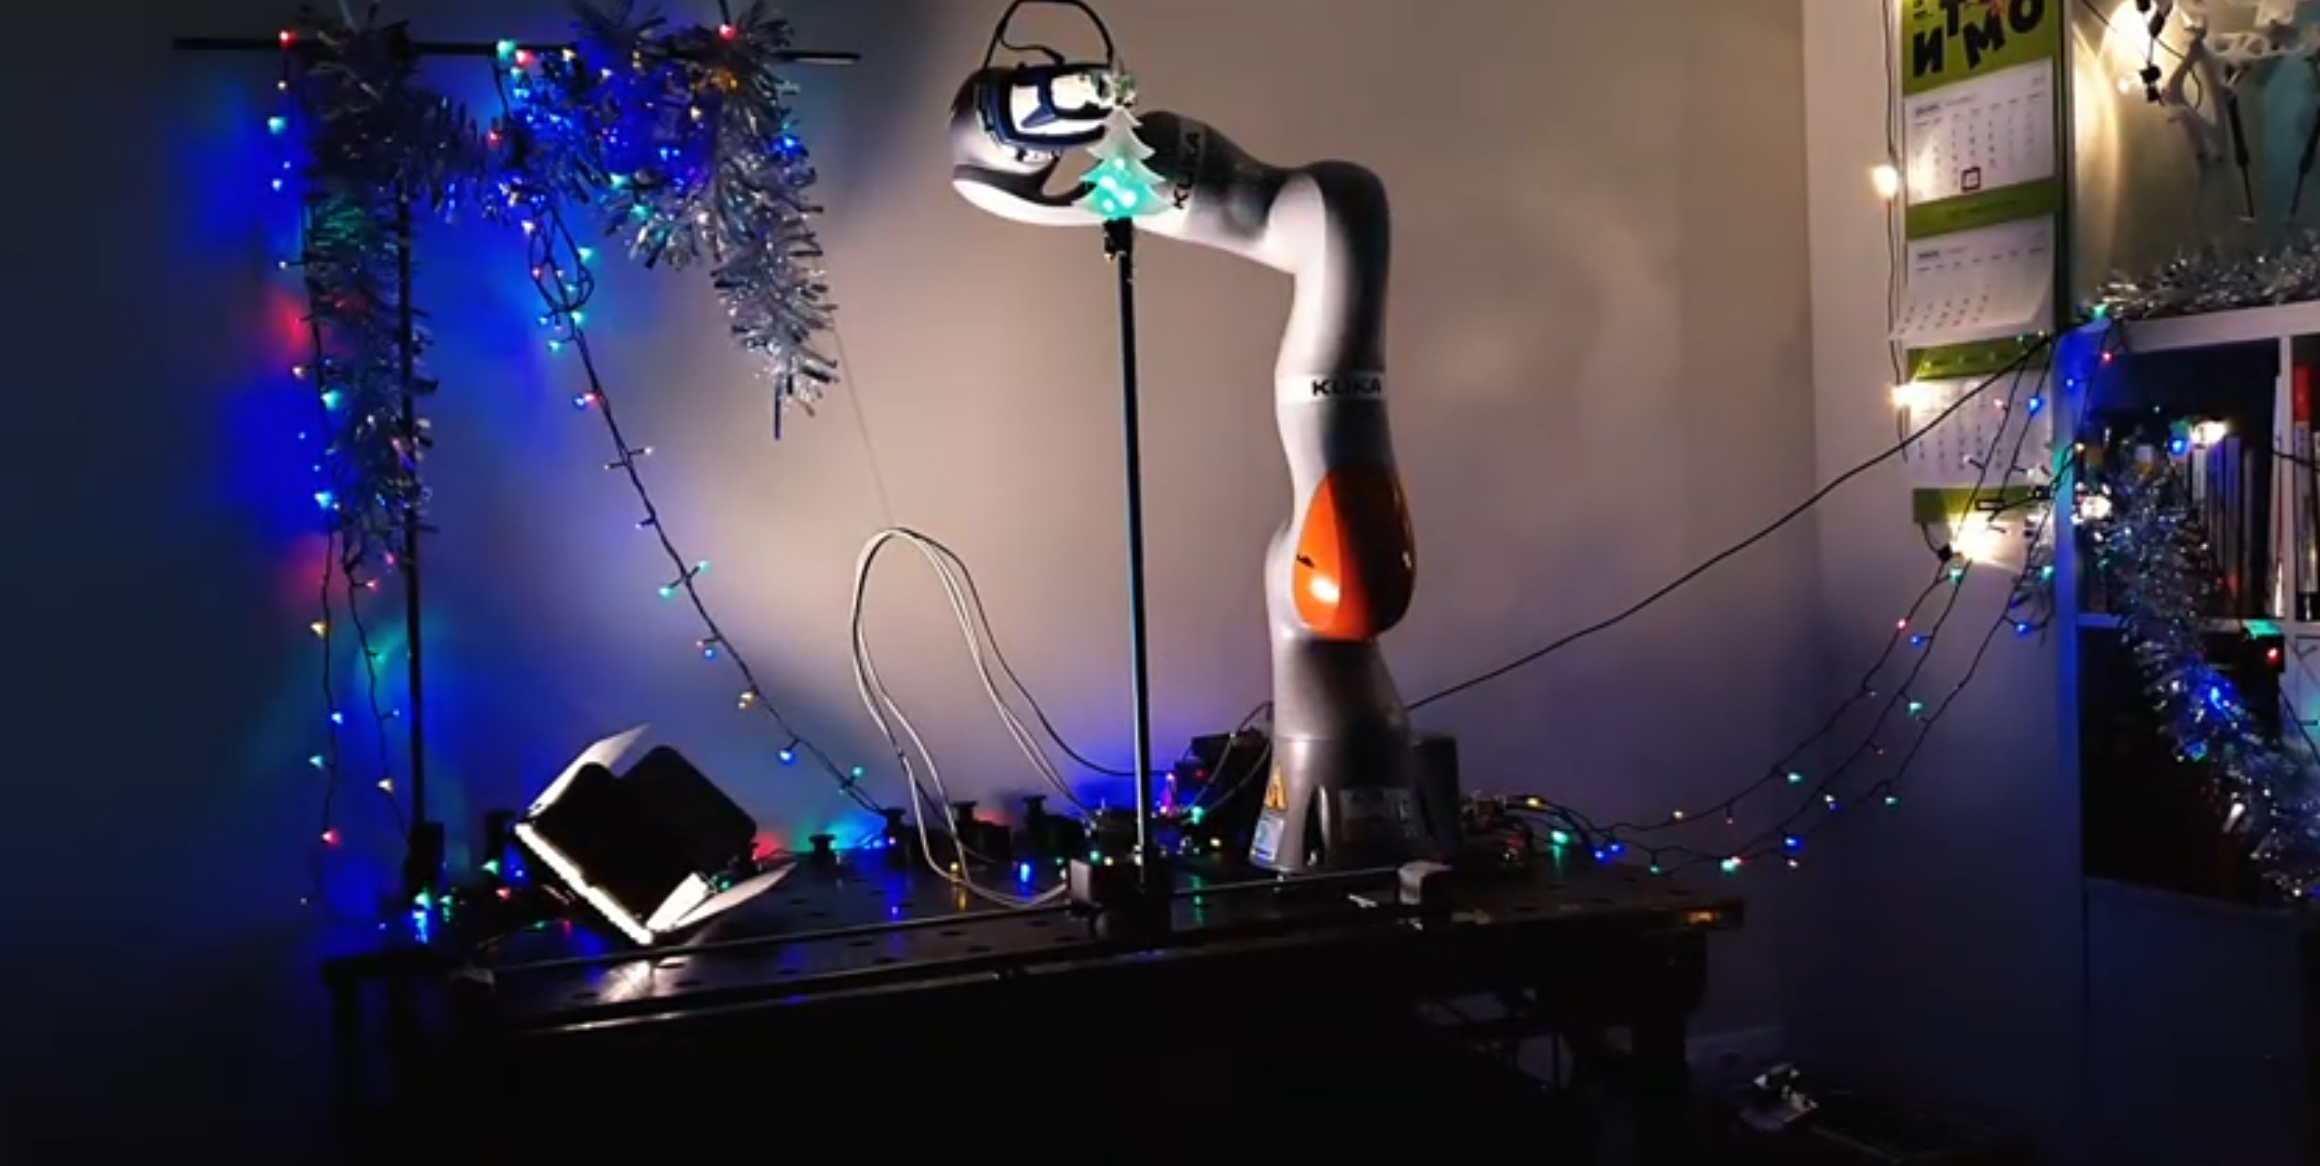
\includegraphics[width=4cm]{figs/tree.png} }}%
    \quad
    \subfloat[\centering Collaborative control of \textbf{FESTO Robotino} and something Drone (\href{https://youtu.be/EBzgKsqisKc}{click})]{{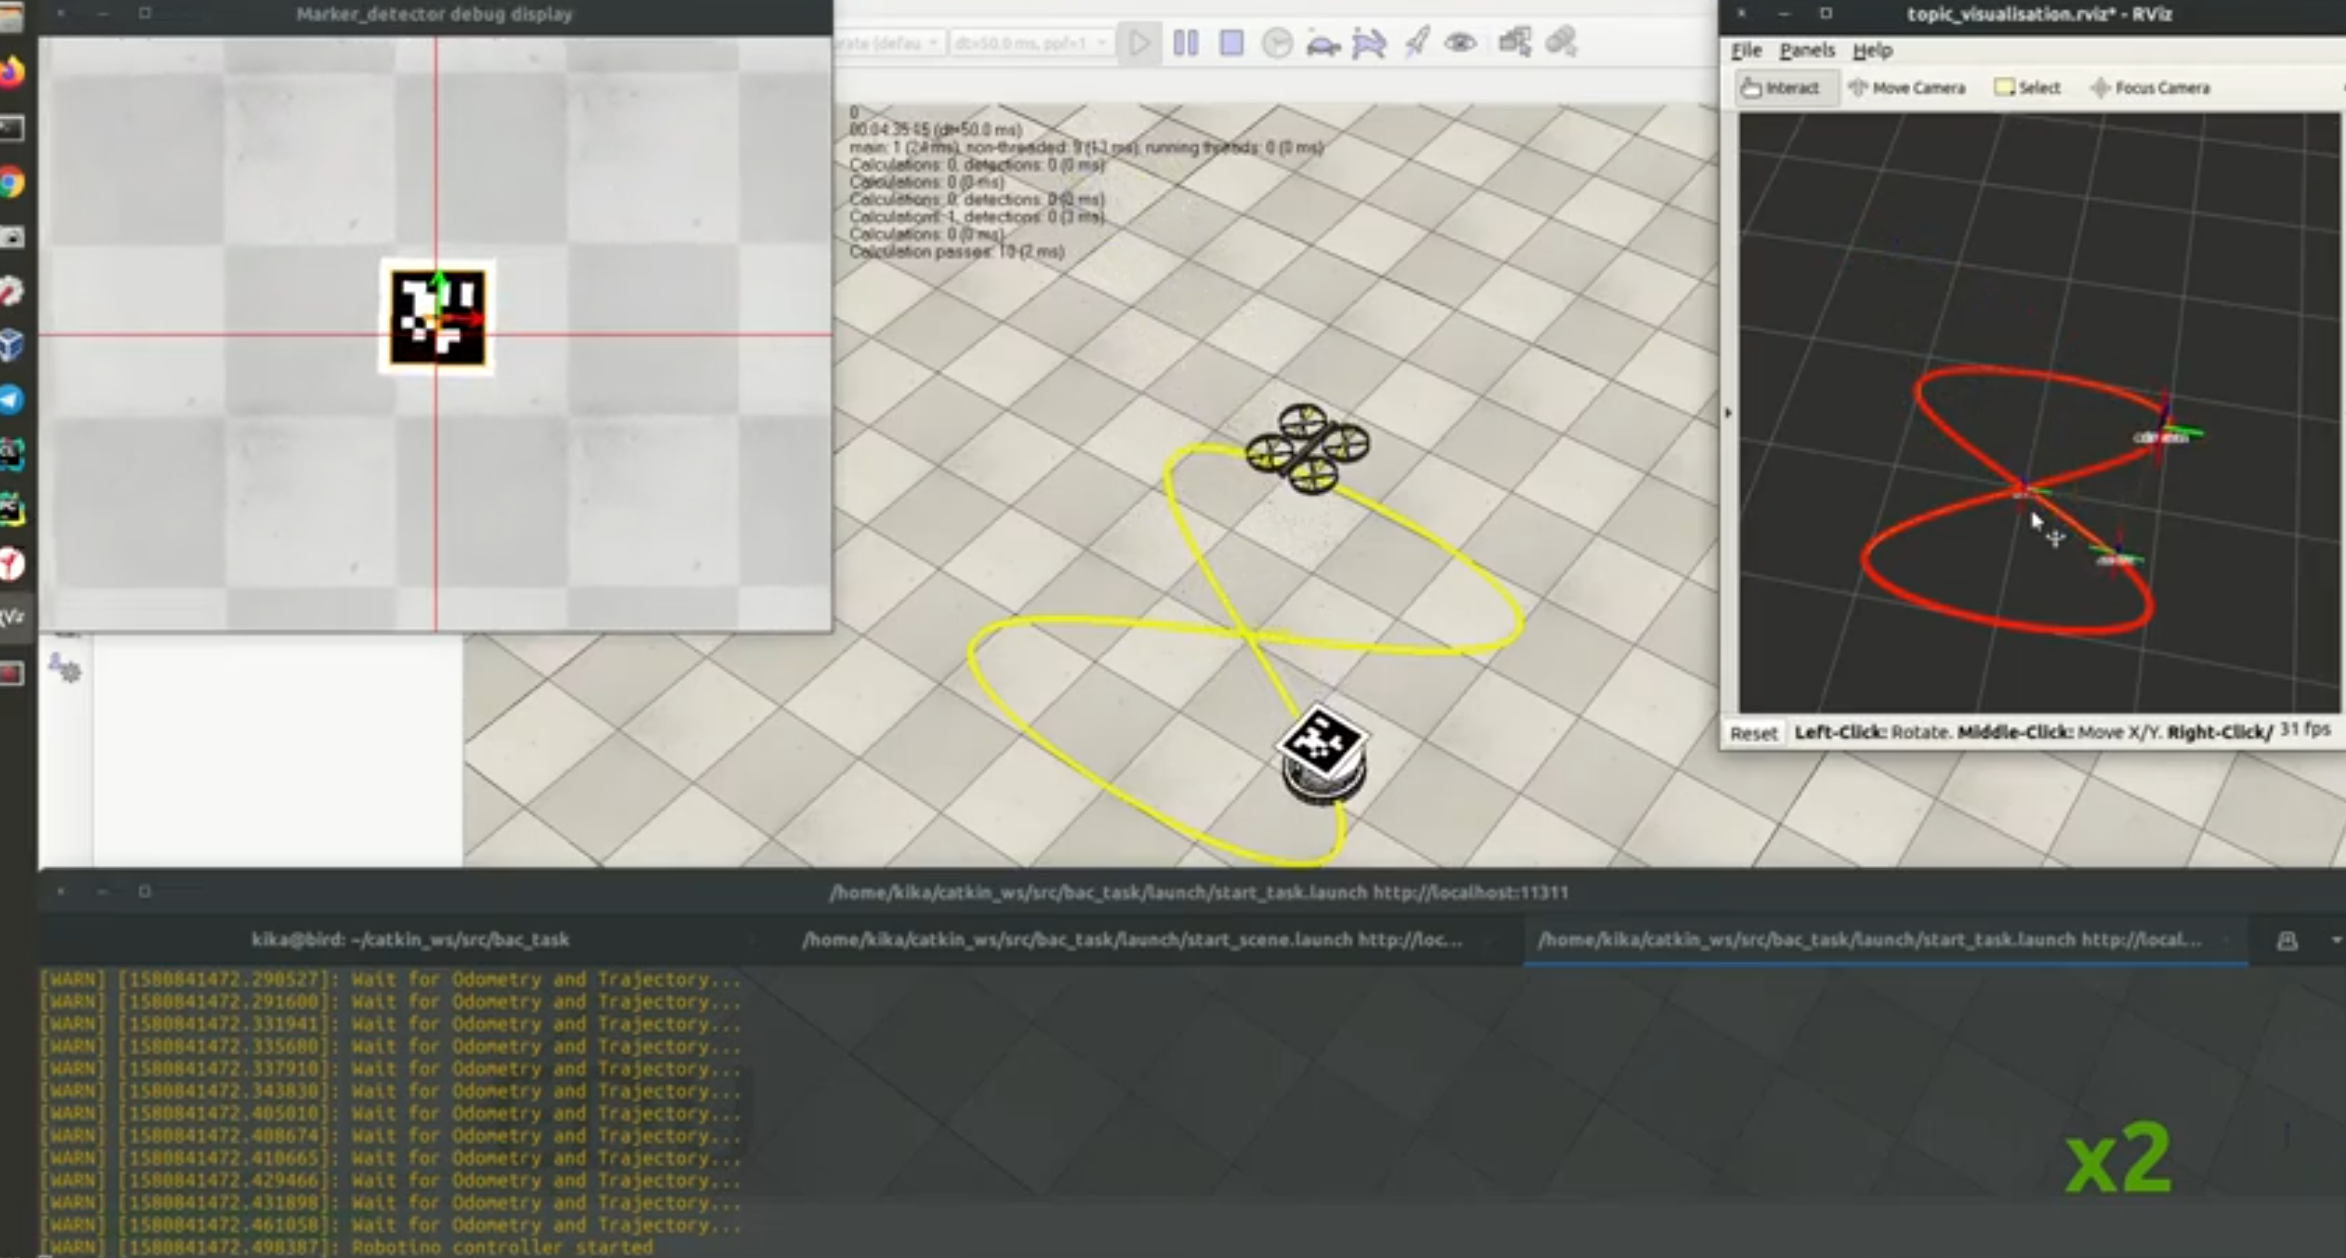
\includegraphics[width=3cm]{figs/yaprofi.png} }}%
    \quad
    \subfloat[\centering Navigation for \textbf{car-like robot (\href{https://youtu.be/3-zPCO2_tgE}{click})}]{{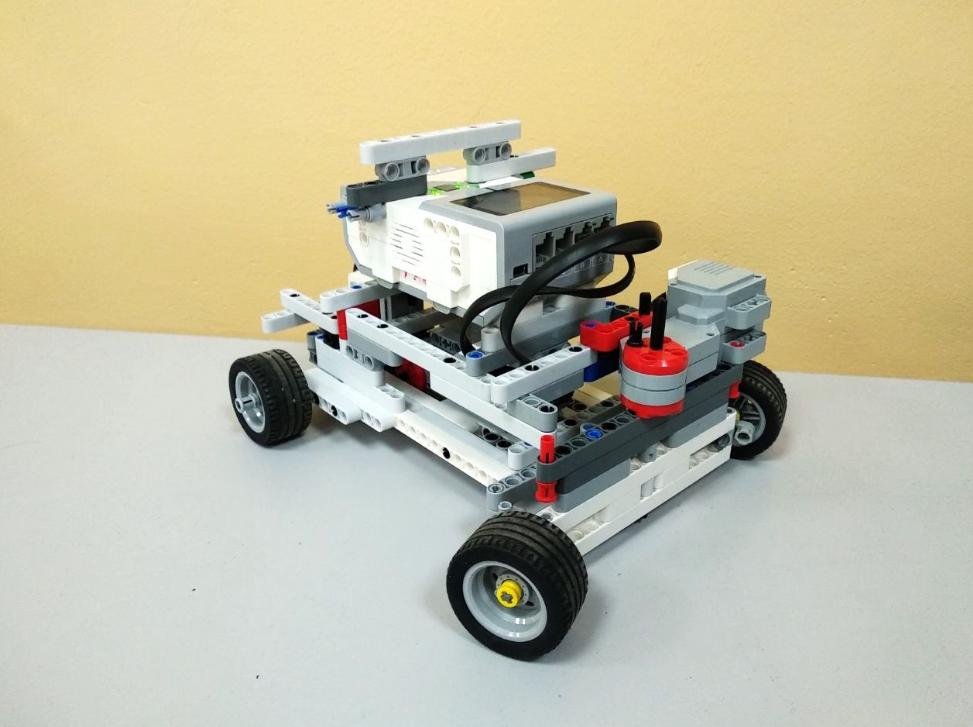
\includegraphics[width=2cm]{figs/car.png} }}%    
\end{figure}

\begin{figure}[h]
    \centering
    \subfloat[\centering Trajectory control by \textbf{KUKA youBot arm (\href{https://youtu.be/sp8Xu5Xg4NM}{click})}]{{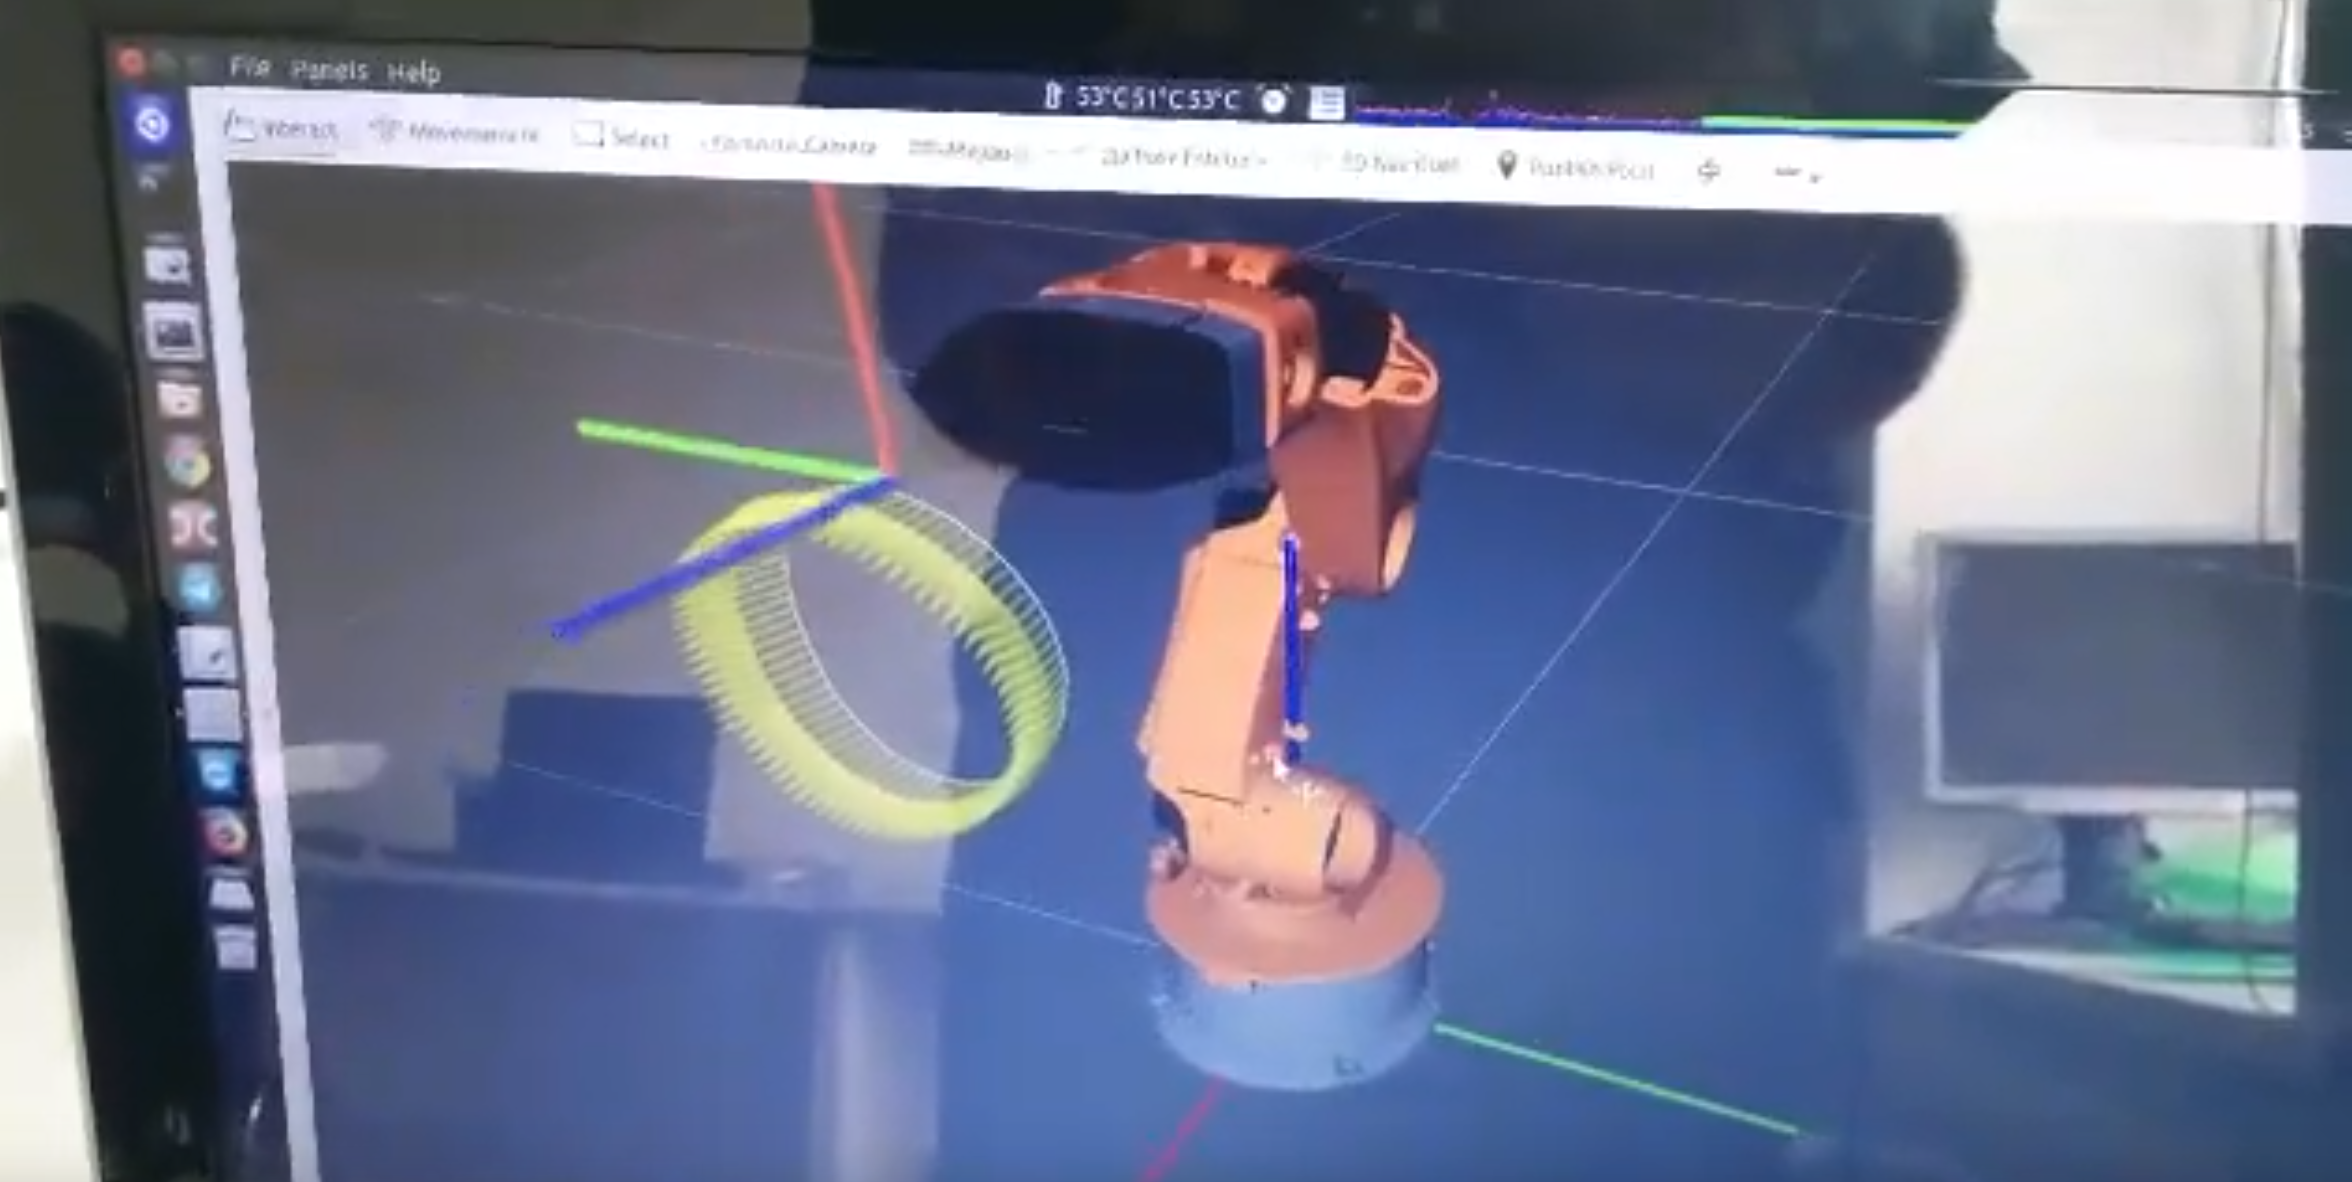
\includegraphics[width=4cm]{figs/traj.png} }}%
    \subfloat[\centering Bottle Cap Challenge by \textbf{KUKA youBot arm (\href{https://youtu.be/JYHDjdC417I}{click})}]{{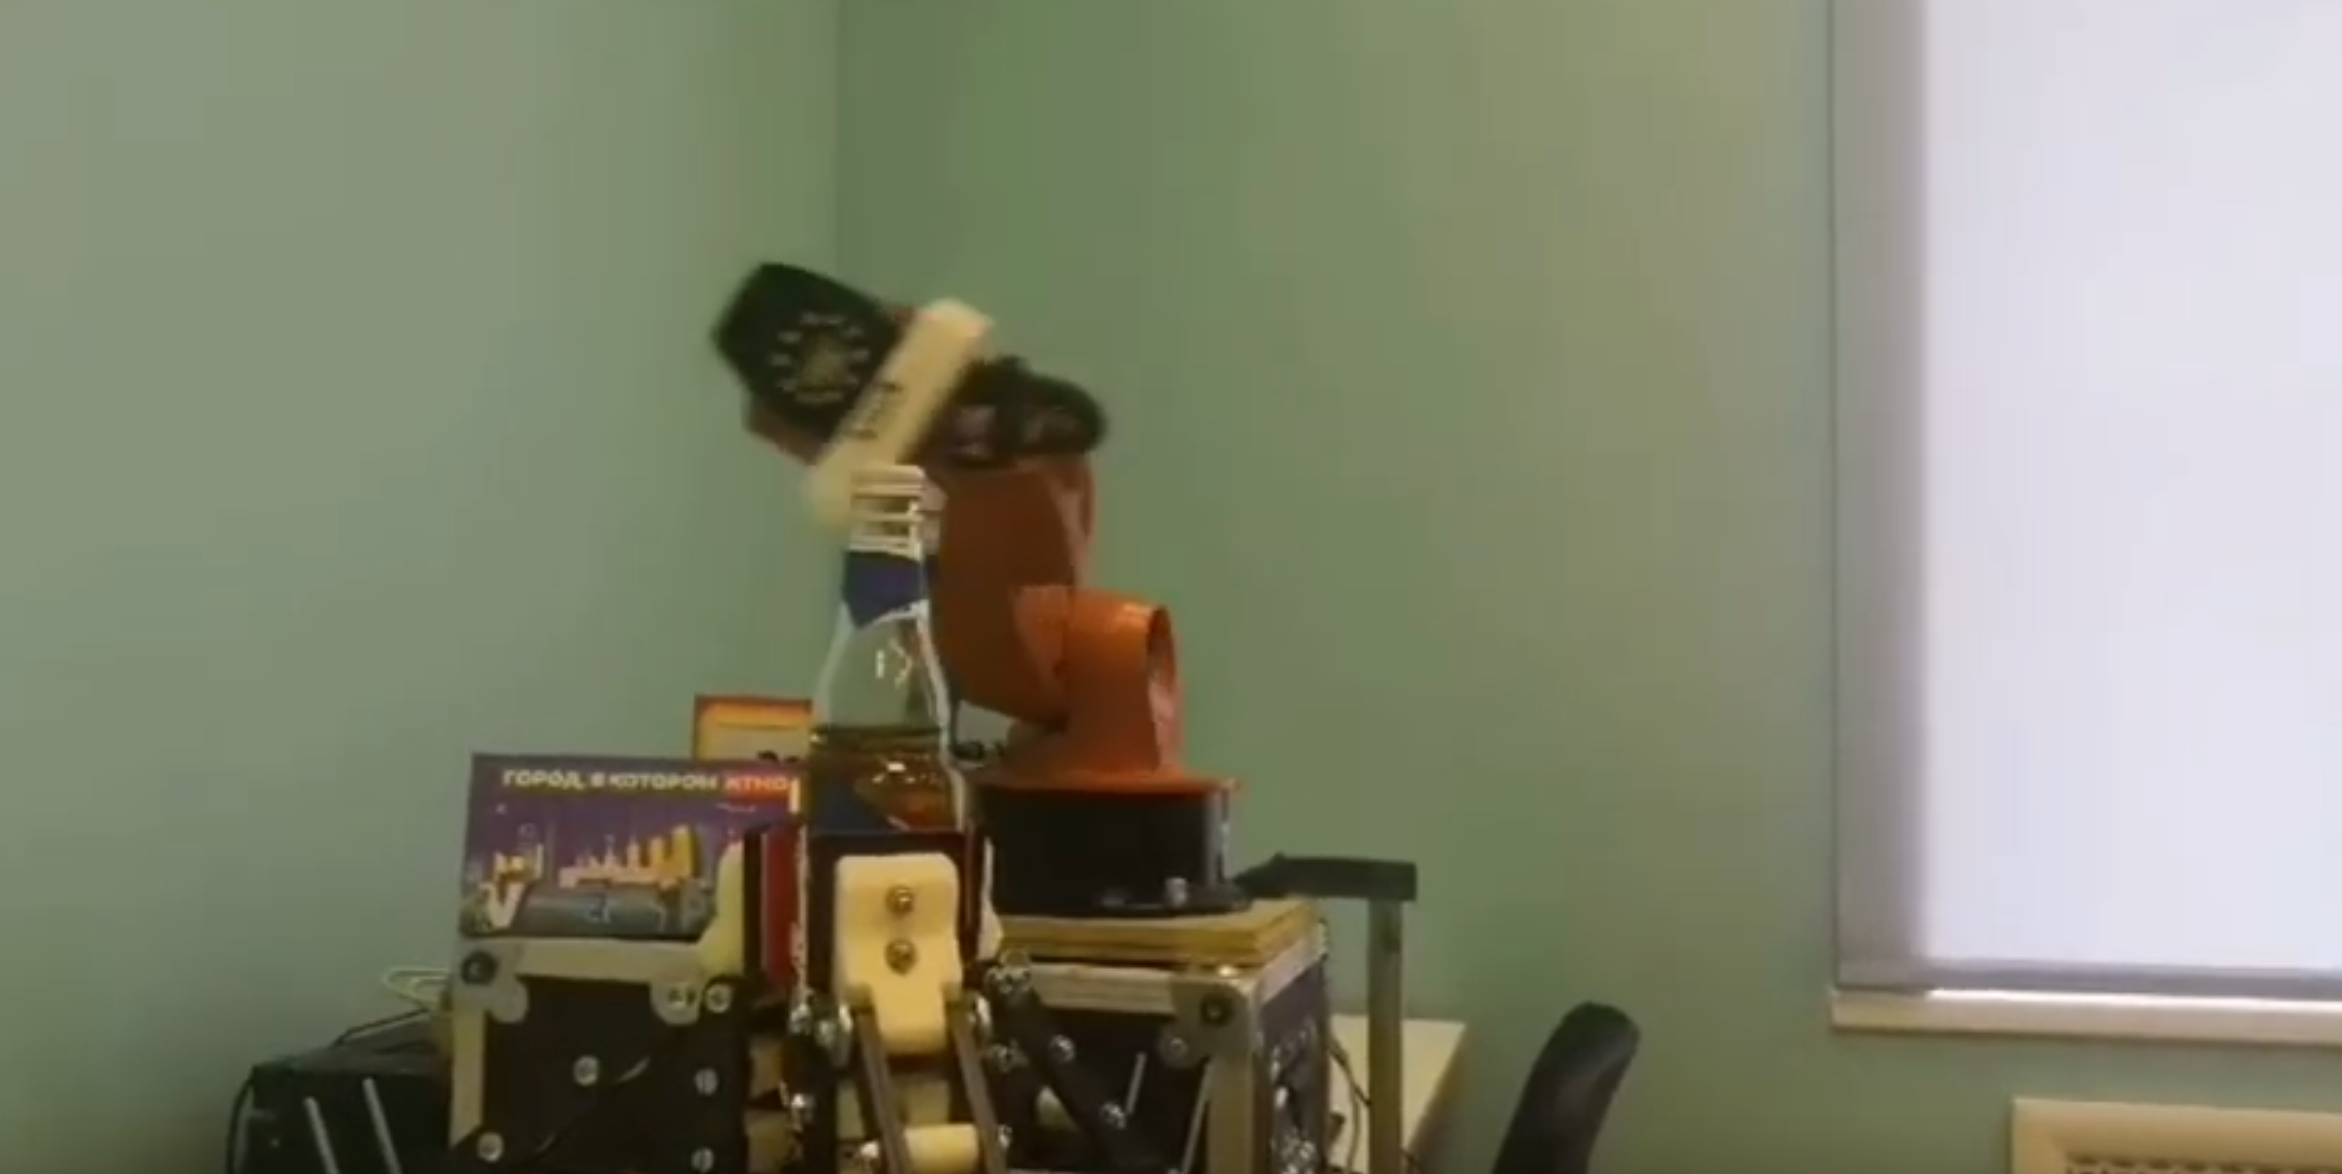
\includegraphics[width=4cm]{figs/cupchallenge.png} }}%
    \quad
    \subfloat[\centering Dynamics parameters identification (\href{https://youtu.be/m_fvHeczBIg}{click})]{{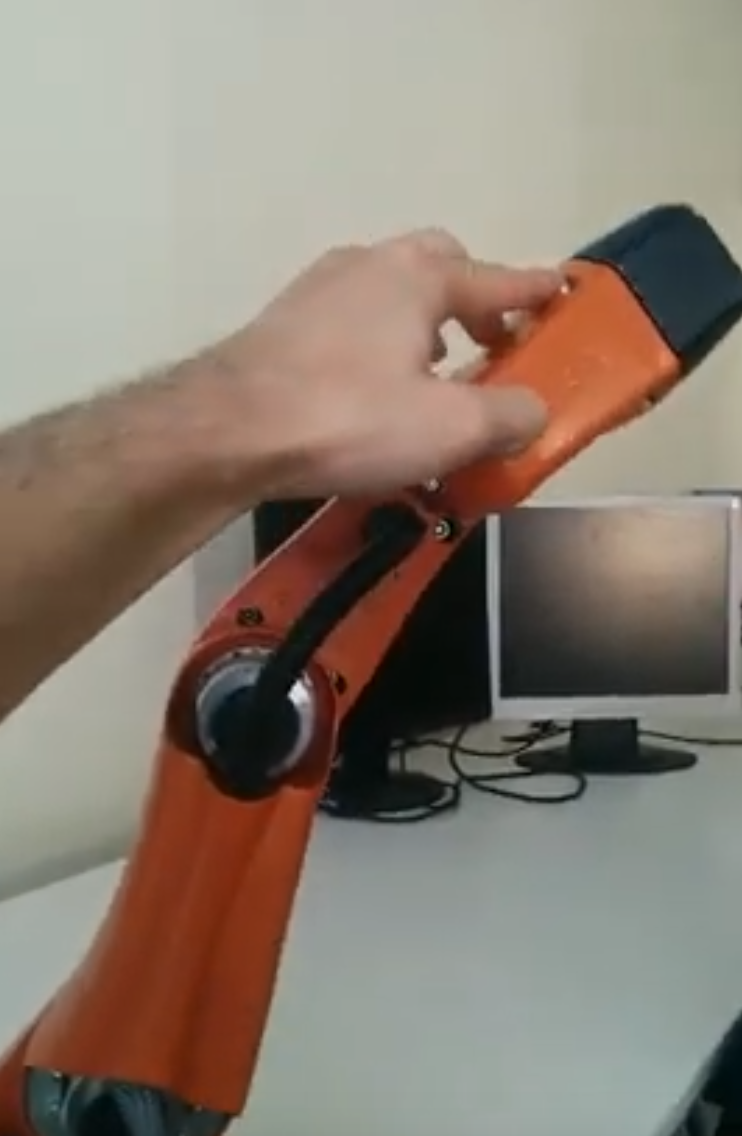
\includegraphics[width=2.8cm]{figs/gravity.png} }}%
    \quad 
    \subfloat[\centering Automatic system for testing robotics competitions in simulators (\href{https://youtu.be/aEhnfeTa0xY}{click})
    ]{{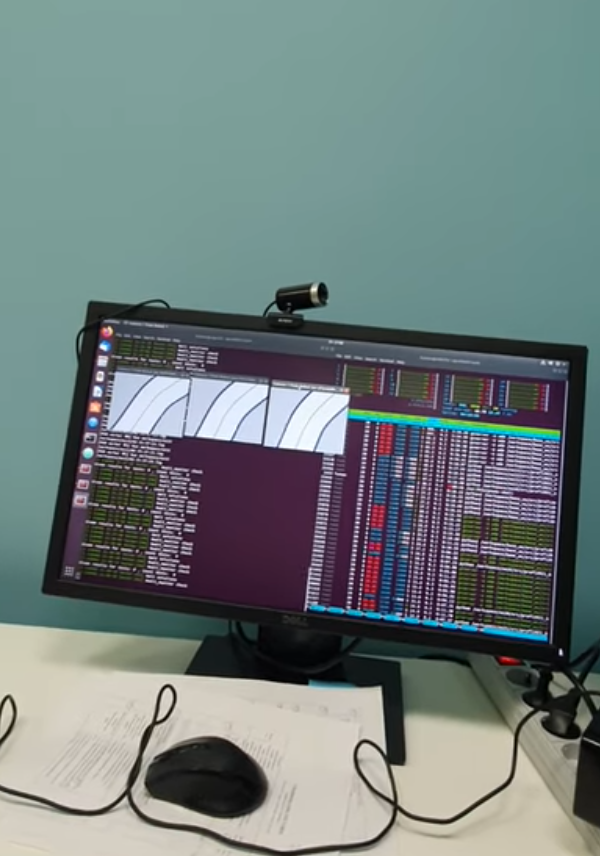
\includegraphics[width=3cm]{figs/testing.png} }}
    \centering
    \subfloat[\centering Velocity control (\href{https://youtu.be/l32D-GiaalY}{click})
    ]{{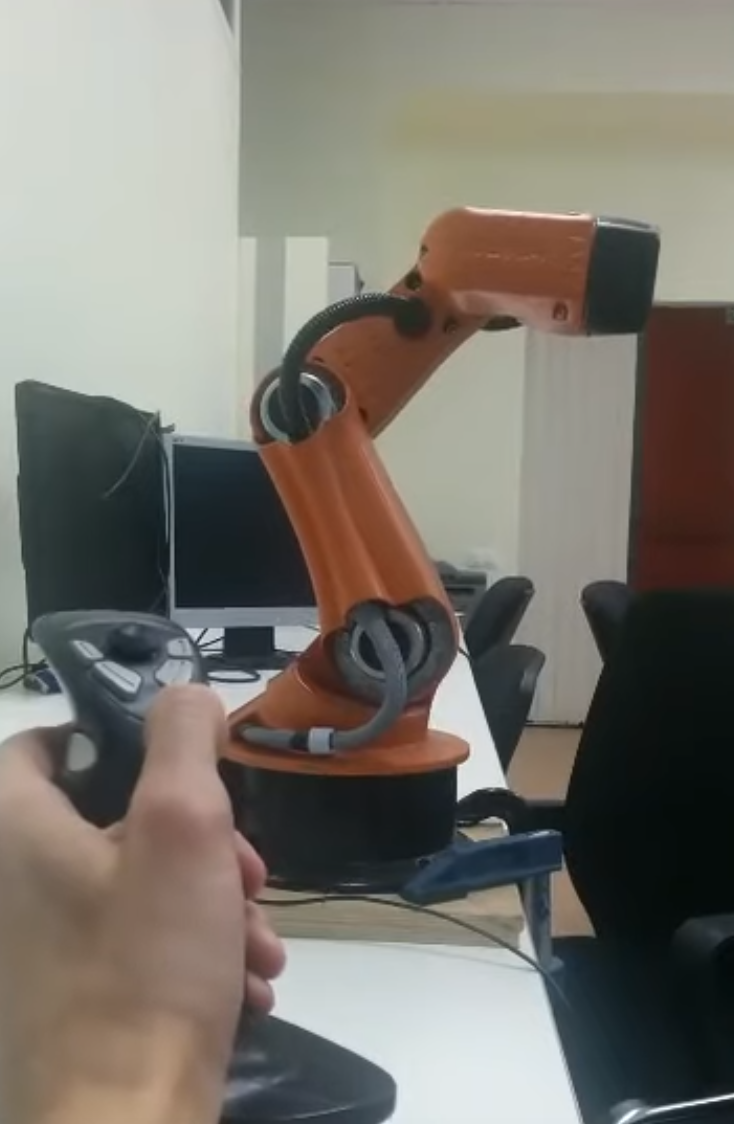
\includegraphics[width=2.8cm]{figs/velcmd.png} }}%
\end{figure}

\end{document}  \documentclass[]{article}
